\begin{problem}[18]{Games: 3-Player Pruning}

\begin{question}[2]{\bf A 3-Player Game Tree}

Consider the 3-player game shown below.  The player going first (at the top
of the tree) is the Left player, the player going second is the Middle
player, and the player going last is the Right player, optimizing the
left, middle and right components respectively of the utility vectors shown.   Fill in the
values at all nodes.  Note that all players \emph{maximize} their
own respective utilities. 
\begin{center}
\solution{ 
    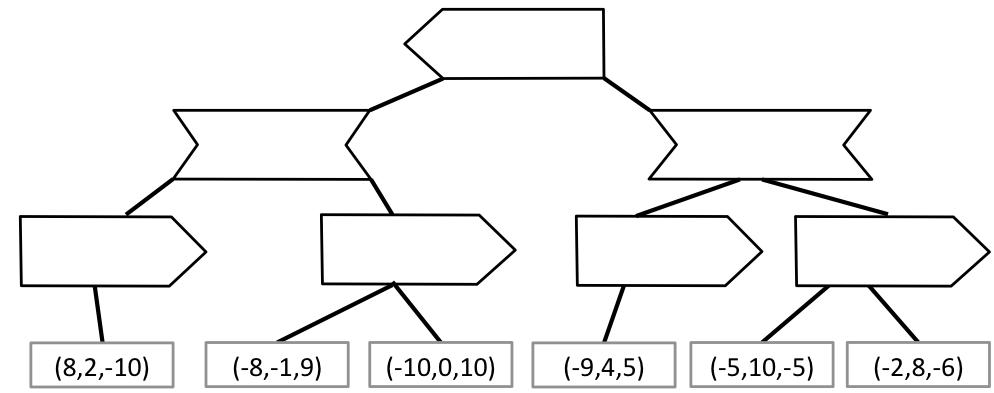
\includegraphics[width=4.5in]{figures/alpha_beta_gamma/abg_q}
} {

    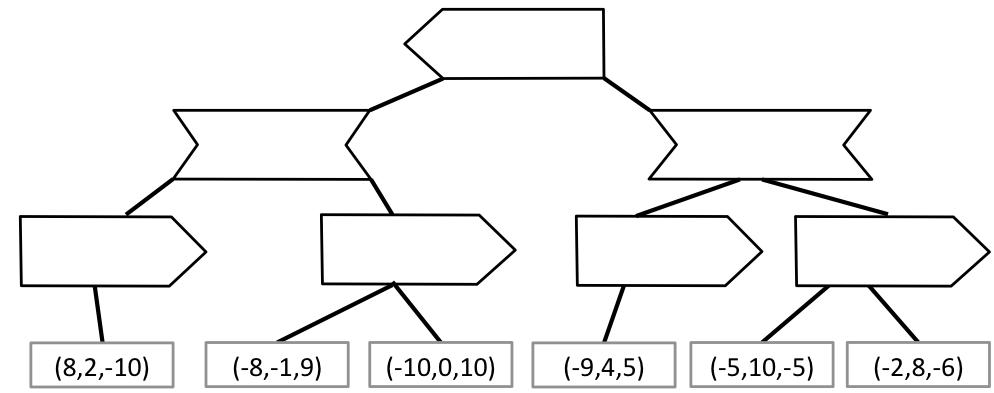
\includegraphics[width=4.5in]{figures/alpha_beta_gamma/abg_q}
  \begin{picture}(0,0)
    \put(-180,110){\OneAroot}
    \put(-260,80){\OneAnodeLeft}
    \put(-100,80){\OneAnodeRight}
    \put(-320,45){\OneAnodeLeftLeft}
    \put(-220,45){\OneAnodeLeftRight}
    \put(-135,45){\OneAnodeRightLeft}
    \put(-65,45){\OneAnodeRightRight}
  \end{picture}

}
\end{center}
\end{question}

\begin{question}[3]{\bf Pruning for a 3-Player Zero-Sum Game Tree}

We would like to prune nodes in a fashion similar to $\alpha$ - $\beta$ pruning.  Assume that we have the knowledge that the sum of the utilities of all 3 players is always zero.
What pruning is possible under this assumption?  Assume the game tree is traversed from left to right. Below, cross off with an $\times$ any branches that can be safely pruned. Justify your answer.

\begin{center}
\solution{
    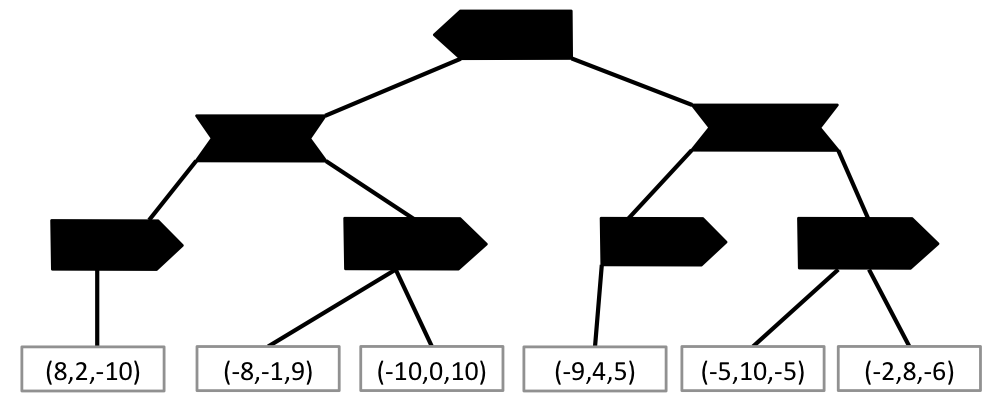
\includegraphics[width=4in]{figures/alpha_beta_gamma/skeleton}
} {\begin{minipage}[b]{25\linewidth}
    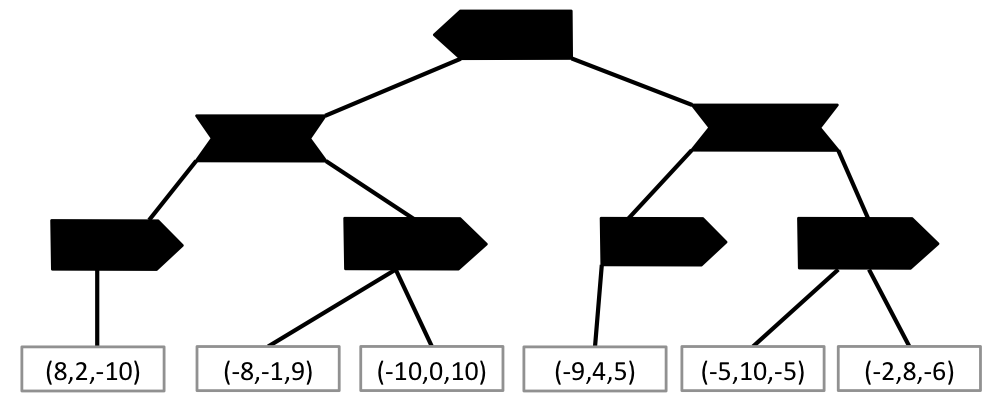
\includegraphics[width=4in]{figures/alpha_beta_gamma/skeleton}
    \begin{picture}(0,0)
    \put(-190,85){\OneBleft}
    \put(-110,85){\OneBright}
    \put(-250,55){\OneBleftleft}
    \put(-190,55){\OneBleftright}
    \put(-110,55){\OneBrightleft}
    \put(-50,55){\OneBrightright}
    \put(-270,20){\OneBleftleftleft}
    \put(-205,20){\OneBleftrightleft}
    \put(-175,20){\OneBleftrightright}
    \put(-125,20){\OneBrightleftleft}
    \put(-70,20){\OneBrightrightleft}
    \put(-40,20){\OneBrightrightright}
    \put(2, 120) {
    
       \fbox{\begin{minipage}[t][4.5cm][t]{7cm} 1b explanation: \OneBExplanation{ }\end{minipage}}
       \\}
    \end{picture}
    \end{minipage}
}
\end{center}
\end{question}

\begin{question}[3]{\bf Pruning for a 3-Player Zero-Sum, Bounded-Utility Game Tree.}

If we assume more about a game, additional pruning may become possible.  Now, in addition to assuming that the sum of the utilities of
all 3 players is still zero, we also assume that all utilities are in the interval $[-10, 10]$.
What pruning is possible under these assumptions? Assume the game tree is traversed from left to right. Below, cross off with an $\times$ any branches that can be safely pruned. Justify your answer.

\begin{center}
\solution{
    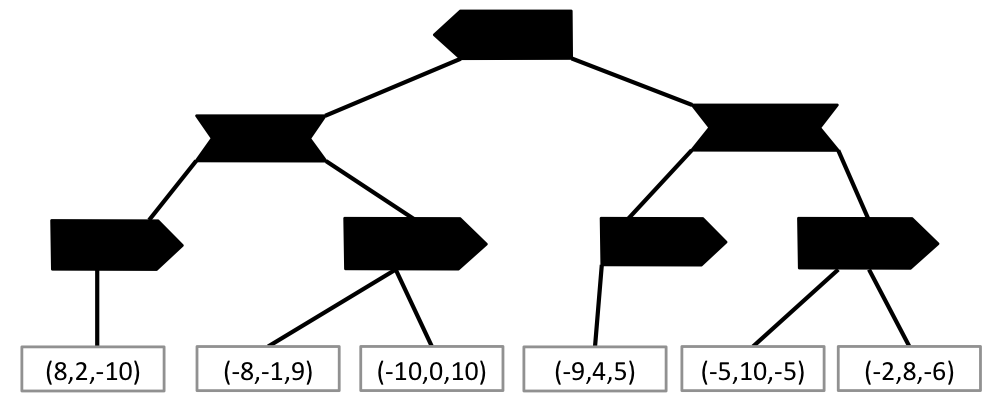
\includegraphics[width=4in]{figures/alpha_beta_gamma/skeleton}
} {
\begin{minipage}[b]{25\linewidth}
    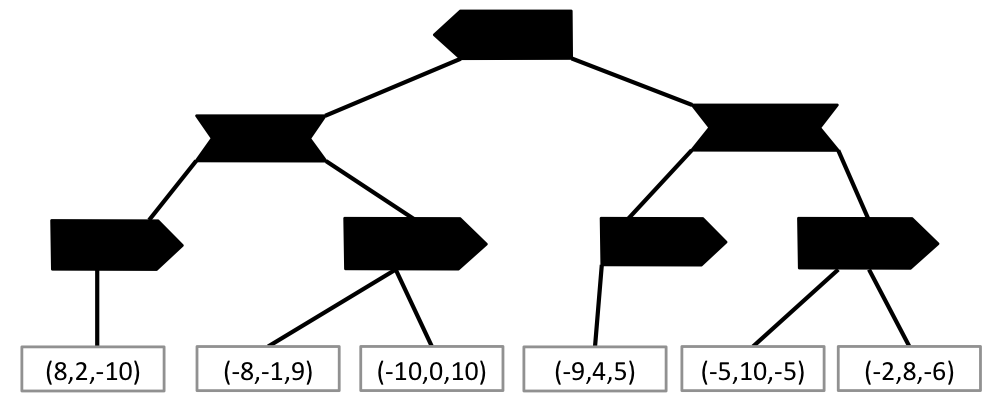
\includegraphics[width=4in]{figures/alpha_beta_gamma/skeleton}
    \begin{picture}(0,0)
    \put(-190,85){\OneCleft}
    \put(-110,85){\OneCright}
    \put(-250,55){\OneCleftleft}
    \put(-190,55){\OneCleftright}
    \put(-110,55){\OneCrightleft}
    \put(-50,55){\OneCrightright}
    \put(-270,20){\OneCleftleftleft}
    \put(-205,20){\OneCleftrightleft}
    \put(-175,20){\OneCleftrightright}
    \put(-125,20){\OneCrightleftleft}
    \put(-70,20){\OneCrightrightleft}
    \put(-40,20){\OneCrightrightright}
        \put(2, 120) {
    
       \fbox{\begin{minipage}[t][4.5cm][t]{7cm} 1c explanation: \OneCExplanation{ }\end{minipage}}
       \\}
    \end{picture}
        \end{minipage}
}
\end{center}

\end{question}
\newpage
\begin{question}[6]{\bf Pruning Criteria}

Again consider the zero-sum, bounded-utility, 3-player game described
above in (c). Here we assume the utilities are bounded by $[-C, C]$ for some constant $C$ (the previous problem considered the case $C=10$). Assume there are only 3 actions in the game, and the order is Left, Middle, then Right. Below is code that computes the utilities at each
node, but the pruning conditions are left out.  Fill in conditions below that prune wherever safe.
\vspace{0.2in}
\begin{subquestion}[2]{\bf Pruning for Left}
\begin{figure}[H]
\begin{minipage}[b]{0.5\linewidth}
\vspace{0.2in}
\begin{verbatim}
Compute-Left-Value(state, C)
  v_L = -infty; alpha = -infty
  for each successor of state:
    (w_L, w_M, w_R) = Compute-Middle-Value(successor, C, alpha)
    if (w_L > v_L)
      v_L = w_L
      v_M = w_M
      v_R = w_R
    end
    // pruning condition:
    if (                 )
      return (v_L, v_M, v_R)
    end
    alpha = max(alpha, v_L)
  end
  return (v_L, v_M, v_R)
\end{verbatim}

\vspace{1in}
\end{minipage}
\raisebox{2.0cm}{
\begin{minipage}[b]{0.5\linewidth}
\centering
Fill in the pruning condition below,
write $false$ if no pruning is possible:

\vspace{0.1in}

\def\arraystretch{3}
\begin{tabular}{|c|}
\hline
\large{\textbf{(}} \solution{\hspace{3.1in}}{
 \OneDiAnswer
}\large{\textbf{)}} \\
\hline
\end{tabular}

\solution{\vspace{0.5in}}{
   \fbox{\begin{minipage}[t][2.5cm][t]{8cm} 1d(i) explanation: \OneDiExplanation \end{minipage}}\\
}
\end{minipage}
}
\end{figure}

\end{subquestion}

\begin{subquestion}[2]{\bf Pruning for Middle}
\begin{figure}[H]
\begin{minipage}[b]{0.5\linewidth}
\vspace{0.2in}
\begin{verbatim}
Compute-Middle-Value(state, C, alpha)
  v_M = -infty; beta = -infty
  for each successor of state:
    (w_L, w_M, w_R) = Compute-Right-Value(successor, C, beta)
    if (w_M > v_M)
      v_L = w_L
      v_M = w_M
      v_R = w_R
    end
    // pruning condition:
    if (                  )
      return (v_L, v_M, v_R)
    end
    beta = max(beta, v_M)
  end
  return (v_L, v_M, v_R)
\end{verbatim}


\end{minipage}
\begin{minipage}[b]{0.5\linewidth}
\centering
Fill in the pruning condition below,
write $false$ if no pruning is possible:



\def\arraystretch{3}
\begin{tabular}{|c|}
\hline
\large{\textbf{(}} \solution{\hspace{3.1in}}{
  \OneDiiAnswer
}\large{\textbf{)}} \\
\hline
\end{tabular}

\solution{\vspace{0.5in}}{
   \fbox{\begin{minipage}[t][2.5cm][t]{8cm} 1d(ii) explanation: \OneDiiExplanation\end{minipage}}\\
}

\end{minipage}
\end{figure}
\end{subquestion}

\newpage
\begin{subquestion}[2]{\bf Pruning for Right}

\begin{figure}[H]
\begin{minipage}[b]{0.5\linewidth}
\vspace{0.2in}
\begin{verbatim}
Compute-Right-Value(state, C, beta)
  v_R = -infty;  gamma = -infty
  for each successor of state:
    (w_L, w_M, w_R) = Evaluate-Utility(successor)
    if (w_R > v_R)
      v_L = w_L
      v_M = w_M
      v_R = w_R
    end
    // pruning condition:
    if (                 )
      return (v_L, v_M, v_R)
    end
    gamma = max(gamma, v_R)
  end
  return (v_L, v_M, v_R)
\end{verbatim}

\end{minipage}
\begin{minipage}[b]{0.5\linewidth}
\centering
Fill in the pruning condition below,
write $false$ if no pruning is possible:

\vspace{0.1in}

\def\arraystretch{3}
\begin{tabular}{|c|}
\hline
\large{\textbf{(}} \solution{\hspace{3.1in}}{
   \OneDiiiAnswer
}\large{\textbf{)}} \\
\hline
\end{tabular}

\solution{\vspace{0.5in}}{
   \fbox{\begin{minipage}[t][2.5cm][t]{8cm} 1d(iii) explanation: \OneDiiiExplanation \end{minipage}}\\

}
\end{minipage}
\end{figure}




\end{subquestion}


\end{question}

\begin{question}[4]{\bf Preparing for the Worst (Case)}

Consider again the game tree from earlier, shown again below. Assume it is not known
whether Middle and Right are rational.  Left wants to
avoid the worst-case scenario according to its own utilities.

\emph{Note: you do not need to fill in this game tree; it is provided purely to aid you in answering the question below.}

\begin{center}
\solution{
    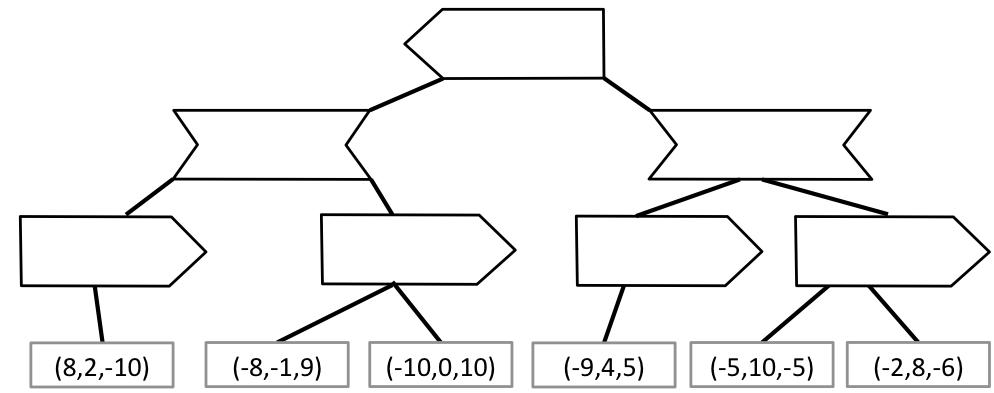
\includegraphics[width=4.5in]{figures/alpha_beta_gamma/abg_q}
} {
    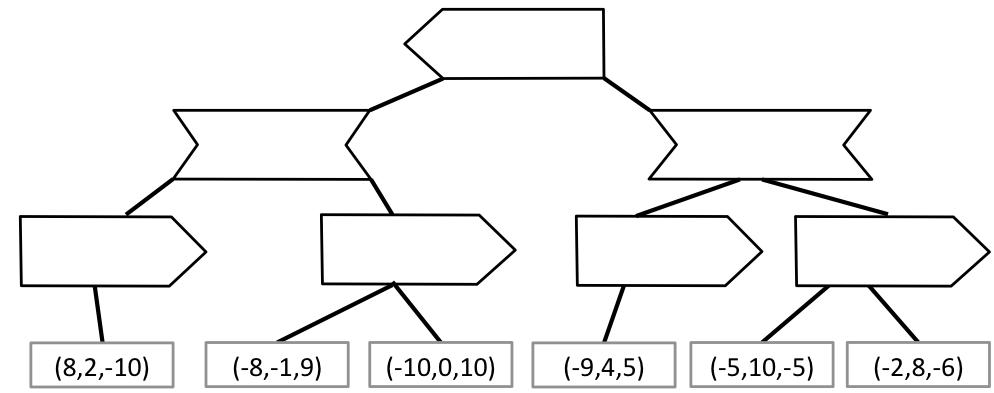
\includegraphics[width=4.5in]{figures/alpha_beta_gamma/abg_q}
}
\end{center}

\begin{subquestion}[2]  What is Left's optimal action? What is the utility achieved in this worst-case scenario?

\solution{\vspace{0.5in}}{
1(e) i answer: \OneEi
}

\end{subquestion}

\begin{subquestion}[2]  Which one of the following approaches would allow,
  for a generic 3-player game, the Left player to compute the strategy
  that optimizes its worst-case outcome? (you may ignore pruning here)

\begin{itemize}[label=]
\OneEii
\end{itemize}

\end{subquestion}
\end{question}
\end{problem}